\documentclass[]{article}
\usepackage{pgfplots}
\usepackage{amsmath}
\usepackage[letterpaper]{geometry}
\geometry{top=0.5in, left=0.6in, right=0.5in, bottom=0.5in}


%opening
\title{MAT 12 CLASS NOTES}
\date{Spring 2016}
\author{Estefany Gebert}

\begin{document}

\maketitle

\tableofcontents
\pagebreak

\section{Types of Numbers}
\subsection{Whole Numbers}
$$ (0,1,2,3,4)$$

\subsection{Natural Numbers}
These are also known as "counting numbers". $$(1,2,3,4...)$$

\subsection{Integers}
Any whole number that does not have decimal or fractional part.
$$(-3,-2,-1,0,1,2,3,4...)$$

\subsection{Even Numbers}
These numbers can be easily divisible by two.
$$(2,4,6,8...)$$

\subsection{Odd numbers}
Number NOT easily divisible by two.
$$(1,3,5,7...)$$

\subsection{Prime Number}
Numbers that are only evenly divisible by themselves or one.\footnote{Two is the only even prime number.}
$$(2,3,5,7,11,13,17,19,23...)$$

\subsection{Irrational Number}
A decimal number that goes on forever and does not repeat. \footnote{$\pi$ is probably the most famous irrational number.}
$$(3.1415926..., \sqrt 2)$$

\subsection{Rational Number}
The opposite of an irrational number. These numbers will eventually end or start repeating.
$$(3.5,3.33333...)$$

\subsection{Number Line}
All real numbers can be found on the number line.

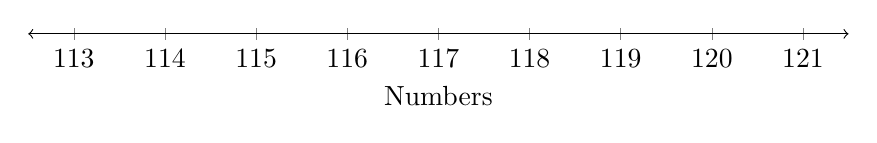
\begin{tikzpicture}
\begin{axis}[
axis y line=none,
axis lines=left,
axis line style={<->},
xmin=112.5,
xmax=121.5,
width=12cm,
height=4cm,
ymin=0,
ymax=1,
xlabel= Numbers,
scatter/classes={o={mark=*}},
restrict y to domain=0:1,
xtick={113,114,...,121}
]
\end{axis}
\end{tikzpicture}

\section{Examples: Types of Numbers}
$$\sqrt {81} = 9 $$
$$\sqrt {49} = 7 $$
$$\sqrt {25} = 5 $$
$$\sqrt {NegativeNumber} = NOT REAL$$ \footnote{Imaginary Numbers are for another lesson.}


\subsection{Simplify}
$$6 \times (7 - 4) \div 3 + 8 - 3 $$
$$6 \times (3) \div 3 + 8 - 3 $$
$$18  \div 3 + 8 - 3 $$
$$6 \div 3 + 8 - 3 $$
$$6 \div 8 - 3 $$
$$14 - 3$$
$$ 11$$


\subsection{Round the Numeral}
\begin{itemize}
	\item 85,379
	\begin{itemize}
		\item Nearest Thousands Place:
		$85,000$
		\item Nearest Tens Place:
		$85,380$
		
	\end{itemize}
\end{itemize}


\subsection{Expanded Notation}
\begin{itemize}
	\item This is the Standard Form: 85,379.
	\item This is the Expanded Notation: 
	
	$$80,000$$
	$$5,000$$
	$$300$$
	$$70$$
	$$9$$
\end{itemize}


\section{Word Problems}
\subsection{Adding}
These are words that you will want to recognize as additoin when reading a Math problem.
\begin{itemize}
\item Add
\item Sum
\item Total
\item Increase
\item Plus
\end{itemize}


\subsection{Subtracting}
Same as addition, these are words to recognoze when reading a word problen dealing with subtraction.
\begin{itemize}
	\item Subtract
	\item Minus
	\item Decrease
	\item Take Away
	\item Less than
	\item from
\end{itemize}


\subsection{Multiply}
Words that point to multiplication. 
\begin{itemize}
	\item Product
	\item Times 
	\item Of	
\end{itemize}
\subsection{Dividing}
Words to be recognized when one needs to divide. 
\begin{itemize}
	\item Divisible
	\item Divide
	\item Division
	\item Quotient
	\item Into
	\item Per
\end{itemize}


\section{Fractions}
These are part of a whole.
\begin{equation*}
	\frac {3}{5} 
\end{equation*}


\subsection{Reducing Fractions}
Common Multiple.
\begin{equation}
	\frac {2 \div 2}{4 \div 2} = \frac{1}{2}
\end{equation}
	\begin{itemize}
		\item 2 = (2,4,6,8,10,12,...)
		\item 4 = (4,8,12,16,20,24,...)
	\end{itemize}
Common Factor.
	\begin{itemize}
		\item 2 = 1,2
		\item 4 = 1,2,4
	\end{itemize}
		2 is the Greatest Common Factor.
\begin{equation}
\frac {8}{24} = \frac {8 \div 8}{24 \div 8} = \frac {1}{3}
\end{equation}


\subsection{Simple Fractions}
\begin{itemize}
	\item Proper: Numerator is smaller than denominator. 
	\begin{itemize}
		\item \begin{equation*}
			\frac{3}{4} 
		\end{equation*}
		\item \begin{equation*}
			\frac{1}{2}
		\end{equation*}
	\end{itemize}
	\item Improper: Numerator ia larger than Denominator. 
		\begin{itemize}
			\item \begin{equation*}
			\frac{4}{3} 
			\end{equation*}
			\item \begin{equation*}
			\frac{2}{1}
			\end{equation*}
		\end{itemize}
\end{itemize}


\subsection{Complex Fractions}
\begin{itemize}
	\item Mixed Numbers:
	\begin{equation}
	3 \frac{2}{5}
	\end{equation}
	\begin{itemize}
		\item Turning Mixed Numbers into an Improper Fraction:
		\begin{equation*}
			W \frac{N}{D} = D \times W + N = \text{Improper Fraction}
		\end{equation*}
	\end{itemize}
	\item Decimals:  3.5, 5.975
\end{itemize}


\subsection{Dividing  Fractions}
\begin{itemize}
	\item Reciprocal "multiplicative inverse"
	\begin{equation*}
		\frac{A}{B} \div \frac{N}{D}  =  \frac{A}{B} \times \frac{D}{B}		
	\end{equation*}
	\item
	\begin{equation}
		\begin{split}
		10 &\div 10 = 1 \\
		10 &\div 5 = 2 \\
		10 &\div 2 = 5 \\
		10 &\div 1 = 10 \\
		10 &\div \frac{1}{2} = 20 \\
		10 &\div \frac{1}{5} = 50 \\
		10 &\div \frac{1}{10} = 100 \\
		10 &\div 20 = \frac{1}{2} \\
		10 &\div 30 = \frac{1}{3} \\
		\end{split}
	\end{equation}
\end{itemize}


\section{Examples: Fractions}
\begin{equation}
	\frac {10+7}{0} = \frac{17}{0}
\end{equation}
\begin{itemize}
	\item Anything Divided by Zero will always be Zero.
\end{itemize}


\subsection{Adding Fractions}
\begin{itemize}
	\item \begin{equation}
	\frac {2}{5} + \frac{3}{5} = 1
	\end{equation}
	\item Same Denominator.
	\begin{equation}
		\frac{5}{8} + \frac{1}{8} = \frac{6}{8} = \frac{3}{4}
	\end{equation}
	\item 
	\begin{itemize}
		\begin{equation}
			\frac{8}{5} + 2 \frac{1}{5} (=INTO>)
			\frac{8}{5} + \frac{11}{5} (=EQUALS=) 
			\frac{19}{5}  (=OR>)  3 \frac{4}{5}
	\end{equation}
\end{itemize}
	\item Different Denominator.
	\begin{equation}
		\frac{1}{2} + \frac{1}{5} = \text{Find LCM}
	\end{equation}
	\item $2 = 2,4,6,8,10... $
	\item $5 = 5,10,15... $
			=10
	\begin{equation}
		\frac{5}{10} + \frac{2}{10} = \frac{7}{5}  \text{Cannot be Reduced}
	\end{equation}
\end{itemize}


\subsection{Subtracting Fractions}
\begin{itemize}
	\item Most of the steps for Subtraction are similar to Addition:
	\item Ex: 1
	\begin{equation}
		\frac{8}{13} - \frac{1}{13} = \frac{7}{13}
	\end{equation}
	\item Ex: 2
	\begin{equation}
		\frac{5}{8} - \frac{3}{8} = \frac{2}{8}
	\end{equation}
	\item Ex: 3
	\begin{align}
	\frac{7}{9} - \frac{2}{3} (=INTO>) \frac{7}{9} - \frac{6}{9} = \frac{1}{9}\\
	\end{align}
	\item Ex: 4
	 \begin{gather*}
	 \text{First turn mixed number into improper fraction.} \\	
		8 \frac{1}{2} - 3 \frac{2}{5} (=INTO>)   \\
		\text{LCM: (2=2,4,6,8,10...),(5=5,10,15...)} \\
		\frac{17 \times 5}{2 \times 5} - \frac{17 \times 2}{5 \times 2} (=INTO>) \frac{85}{10} - \frac{34}{10} (=EQUALS>) \frac{51}{10}\\
		\text{This answer can be turned into a Proper Fraction(Mixed Number)} \\
		= 5 \frac{1}{10}
	\end{gather*}
\end{itemize}

\section{Exponents}
\begin{itemize}
	\item An exponent is a quantity representing the power to which a given number or expression is to be raised, usually expressed as a raised symbol beside the number or expression (e.g., 3 in 23 = 2 x 2 x 2).
	\item \begin{equation}
		(\frac{2}{5}) ^3 (=INTO>) ( \frac{2}{5} ) \times ( \frac{2}{5} ) \times ( \frac{2}{5} ) = \frac{8}{125} (\text{No GCF, Cannot be Reduced})
	\end{equation}
	\begin{itemize}
				\item Base = $ \frac{N=2}{D=3} $
				\item Exponent(power) = 3
	\end{itemize}
	\item \begin{equation}
		(\frac{4}{9})^2 (=INTO>) (\frac{4}{9}) \times (\frac{4}{9}) = \frac{16}{81} (\text{No GCF})
	\end{equation}
	\item \begin{equation}
		(\frac{2}{8})^3 (=INTO>) (\frac{2}{8}) \times (\frac{2}{8}) \times (\frac{2}{8}) = \frac{1}{64}
	\end{equation}
	\begin{itemize}
		\item OR: Reduce First
		\begin{equation}
			(\frac{1}{4}) (=INTO>) (\frac{1}{4}) \times (\frac{1}{4}) \times (\frac{1}{4}) = \frac{1}{64}
		\end{equation}
	\end{itemize}
\end{itemize}

\section{Prime Factors}
\begin{itemize}
	\item A Prime Factor is...
\end{itemize}

\subsection{Ugh I'm Sleepy...}




\end{document}
